% -----------------------------------------------------------
\chapter{Funciones de orden superior, closures e iteradores}
\label{ch_funciones}
% -----------------------------------------------------------

\begin{Resumen}
   En matemáticas y en ciencias de la computación, se denominan funciones de orden superior a las que cumplen al menos una de las siguientes condiciones:
   
   \begin{itemize}
      \item Tomar una o más funciones como parámetro de entrada.
      \item Devolver una función como salida.
   \end{itemize}
   
   En matemáticas, un ejemplo lo podría constituir la función derivada, que toma una función como parámetro y devuelve otra función.
   
   \smallskip
   
   En programación funcional, las funciones son consideradas elementos de primera clase, esto es, pueden usarse como argumentos de otras funciones, como valores devueltos y también asignarse a un símbolo o variable. La mayoría de los lenguajes han adoptado ya esta premisa y dan un tratamiento de primera clase a las funciones.
   
   \smallskip
   
   En este capítulo se va a hablar de funciones, de cómo asignarlas a variables y de cómo  utilizarlas como argumento o como valor devuelto de otras funciones.
   
   \smallskip
   
   También se hablará de las closures, que son un tipo especial de funciones definidas dentro de otras funciones, que pueden acceder al contexto en el que se han definido. 
   
   \smallskip
   
   Por último, se hablará de los iteradores y cómo encadenar procesos utilizando iteradores y funciones de orden superior.
   
\end{Resumen}

\section{Funciones de primera clase}
\noindent En programación, se denominan \textit{elementos de primera clase} a los elementos del lenguaje que se pueden asignar a variables y se pueden utilizar como argumentos o como valor devuelto por otras funciones.

No todos los elementos del lenguaje son elementos de primera clase. Por ejemplo, en muchos lenguajes, los operadores aritméticos como el $+$, el $-$ y otros, no son de primera clase. También sucede algo parecido con algunas construcciones, como los bucles o las bifurcaciones.

Es importante entender la diferencia entre el concepto de \textit{declaración} y el de \textit{expresión}. Un elemento de un lenguaje se considera que es una \textit{declaración} cuando no devuelve ningún valor; una \textit{expresión}, en cambio, es un elemento que devuelve un valor.

En los lenguajes funcionales se da prioridad a las expresiones que devuelven valores. Así se hace en Rust. Algunas construcciones que en otros lenguajes son declaraciones, en Rust son expresiones. Es el caso de las bifurcaciones \textit{if} o de los bucles \textit{loop, for} o \textit{while}, como se indicó en los apartados \ref{sec_bifurcaciones} y \ref{sec_bucles}. En cambio, el operador \textit{let} es una declaración que no devuelve ningún valor.

Se podría realizar un código como el siguiente:

\vspace{0.7em}
\begin{Codigo}
   fn main() {
      let x = 2;
      println!("{}", suma(if x==2 {3} else {4}, 5));
      
      let mut n = 1;
      println!("{}", loop {
         n=n+1;
         if n>3 {
            break 10
         }
      });
   }
   fn suma(x: i32, y: i32) -> i32 {
      x+y
   }
\end{Codigo}

En el programa anterior, se utiliza una bifurcación \textit{if} como argumento de la función \textit{suma()} y un bucle \textit{loop} como argumento de la macro \textit{println!()}. Observe que, en realidad, el argumento es el valor que devuelven dichas expresiones. 

Actualmente, numerosos lenguajes se han adherido a la línea marcada por los lenguajes funcionales y consideran las funciones como elementos de primera clase, esto es, permiten que las funciones se puedan asignar a variables y se puedan utilizar como parámetros o como valor devuelto por otras funciones. En Rust, las funciones son objetos de primera clase.

Se denominan \textit{funciones de primer orden} o también \textit{funciones ordinarias} aquellas en las que ni los parámetros ni el valor devuelto son otras funciones. Por contra, las \textit{funciones de orden superior} son aquellas en las que o bien alguno de los parámetros o bien el valor devuelto son una función.

Hay varias maneras de definir funciones en Rust:

\begin{itemize}
   \item Dentro de un módulo o fichero \textit{.rs}, con la visibilidad que le corresponda y acceso a otras funciones y a sus variables locales .
   \item Dentro de otra función o bloque de código, con visibilidad restringida a dicho bloque y acceso a otras funciones, pero no a variables del contexto del bloque en el que se ha definido.
   \item Cómo función asociada a un tipo de datos personalizado, como es el caso de las estructuras y las enumeraciones.
   \item Como closure definida dentro de otra función o bloque de código. Su visibilidad estará restringida al bloque en el que se ha definido, pero las closures sí que tienen acceso a las variables existentes en el contexto del bloque en el que se haya definido. 
\end{itemize}

Ya se comentó este tema en el Apartado \ref{sec_funciones}. También se habló allí de los tres tipos de funciones que considera Rust, en función del uso que hacen de la propiedad de los parámetros: el tipo \textit{Fn}, para funciones ordinarias, el tipo \textit{FnMut}, para funciones con parámetros mutables y el tipo \textit{FnOnce} para funciones que solo se pueden invocar una vez.

\subsection{Asignación de funciones a variables}
\noindent Cualquiera de los tipos de funciones presentes en Rust se pueden asignar a una variable. Luego, se puede utilizar la variable como si fuera la función. 

El siguiente código asigna a una variable de nombre \textit{raiz2} la función \textit{sqrt} de los números \textit{f64}. Como resultado, la variable \textit{raiz2} es del tipo \textit{fn(f64) -> f64}, esto es, una función que recibe un argumento del tipo \textit{f64} y devuelve un valor \textit{f64}. Observe la forma de calcular la raíz cuadrada utilizando la variable así definida:

\vspace{0.7em}
\begin{Codigo}
   fn main() {
      let raiz2  = f64::sqrt;
      let y = raiz2(4.0); // Equivale a 4.0f64.sqrt()
      println!("{}", y);
   }
\end{Codigo}

Se podría asignar una función previamente codificada, como se hace en el siguiente código:

\vspace{0.7em}
\begin{Codigo}
   fn main() {
      let f = saludo;
      f(); // Imprime Hola, ¿qué tal?
   }
   fn saludo() {
      println!("Hola, ¿qué tal?");
   }
\end{Codigo}

En este caso, la variable \textit{f} es del tipo \textit{fn()}, esto es, del tipo de las funciones que no reciben argumentos y no devuelven ningún valor.

Las closures también se pueden asignar a variables, como se hace en el siguiente ejemplo:

\vspace{0.7em}
\begin{Codigo}
   fn main() {
      let cuadrado = |x| x*x;
      println!("{}", cuadrado(3.0)); // Imprime 9
   }
\end{Codigo}

Este tipo de funciones que no se definen dentro de un bloque \textit{fn} con nombre, se denominan \textit{funciones anónimas}. En este caso, la función anónima se ha asignado a la variable \textit{cuadrado}. 

También se suele decir que la closure se ha codificado \textit{inline}. El término \textit{inline} se refiere a que la codificación de la función se ha hecho dentro de la línea de código de otra instrucción. Es habitual también codificar closures \textit{inline} cuando se utilizan como parámetros de otras funciones.

\pagebreak
\subsection{Utilización de funciones como parámetros de otras funciones}
\noindent Observe el código siguiente:

\vspace{0.7em}
\begin{Codigo}
   fn main() {
      let pi = std::f64::consts::PI;
      println!("{}", operador(f64::sin, pi/2.0)); // Imprime 1
      println!("{}", operador(f64::cos, pi)); // Imprime -1
      println!("{}", operador(|x| x*x, 4.0)); // Imprime 16
      println!("{}", operador(duplica, 5.0)); // Imprime 10
   }
   fn operador(f:fn(f64) -> f64, x: f64) -> f64 {
      f(x)
   }
   fn duplica(x: f64) -> f64 {
      x*2.0
   }
\end{Codigo}

En el código anterior, la función \textit{operador} es una función de orden superior que se ha definido con la siguiente signatura:

{\centering \texttt{fn operador(f:fn(f64) -> f64, x: f64) -> f64} \par}

Cualquier función con un único parámetro del tipo \textit{f64} y que devuelve un valor del tipo \textit{f64}, se podrá utilizar como argumento en la llamada a la función \textit{operador()}. La función \textit{operador()} devolverá el resultado de aplicar la función \textit{f} que recibe como primer argumento al valor \textit{x} del tipo \textit{f64} que recibe como segundo argumento.

En algunos lenguajes, a la función que se pasa como argumento, para que la función de orden superior la invoque, se le denomina \textit{función de callback}. 

\subsection{Uso de funciones como valor devuelto por otras funciones}
\noindent En el siguiente código se define una función de orden superior, llamada \textit{operador}, que recibe un número entero como argumento. Si el valor recibido es mayor que cero, \textit{operador()} devuelve la función \textit{f64::sin}; en caso contrario, devuelve la función \textit{f64::cos}.

\vspace{0.7em}
\begin{Codigo}
   fn main() {
      let pi = std::f64::consts::PI;
      let seno = operador(3);
      println!("{}", seno(pi/2.0)); // Imprime 1
      let coseno = operador(-2);
      println!("{}", coseno(pi)); // Imprime -1
   }
   fn operador(n: i32) -> fn(f64) -> f64 {
      if n>0 {f64::sin} else {f64::cos}
   }
\end{Codigo}

Otra forma de indicar el tipo de función que se pasa como parámetro o que se devuelve como resultado es utilizar la cláusula \textit{impl} y el nombre del \textit{Trait}, que en este caso es parecido pero poniendo \textit{Fn} en mayúsculas:

{\centering \texttt{fn operador(n: i32){ }->{ }impl Fn(f64) -> f64} \par}

\section{Errores de ejecución}
\noindent El mecanismo de excepciones es la forma habitual que ofrecen muchos lenguajes para gestionar los errores que se producen durante la ejecución de los programas. Pueden ser errores debidos a la entrada de un dato incorrecto, al intento de acceso a un fichero que no existe, el intento de acceder a una página web sin tener conexión u otros tipos de errores de ejecución. En muchas ocasiones, el error de ejecución proviene de la existencia de un puntero nulo en alguna parte del programa.

El invento del puntero nulo se atribuye a Tony Hoare, durante la implementación de los tipos de datos para el lenguaje ALGOL W, a mediados de la decada de 1960. Años después, él mismo lo llamó \textit{el error de los mil millones de dólares}\footnote{Esta cita se ha tomado de la Wikipedia}:
\begin{center}
   \begin{minipage}{0.8\textwidth}
      \itshape\small
      \hspace{1em}``I call it my billion-dollar mistake. It was the invention of the null reference in 1965. At that time, I was designing the first comprehensive type system for references in an object oriented language (ALGOL W). My goal was to ensure that all use of references should be absolutely safe, with checking performed automatically by the compiler. But I couldn't resist the temptation to put in a null reference, simply because it was so easy to implement. This has led to innumerable errors, vulnerabilities, and system crashes, which have probably caused a billion dollars of pain and damage in the last forty years.''
   \end{minipage}
\end{center}

\vspace{1em}
En Rust no existe el puntero \textit{null}. Tampoco existe un mecanismo de excepciones para el tratamiento de los errores de ejecución. En Rust se distingue entre dos tipos de errores de ejecución:

\begin{itemize}
   \item \textit{Errores recuperables}: por ejemplo, se pide al usuario el nombre del fichero que se pretende abrir y se comprueba que dicho fichero no existe. En esos casos, lo que se puede hacer es informar del error al usuario y volver a pedirle el nombre del fichero.
   \item \textit{Errores no recuperables:} por ejemplo, se necesita acceder a un dispositivo y el dispositivo no existe. En estos casos se interrumpe la ejecución del programa, quizás imprimiendo un mensaje que informa al usuario del error que se ha producido.
\end{itemize}

En Rust, cuando el error da lugar a la interrupción del programa se suele decir que el programa \textit{ha entrado en pánico}, por analogía con el nombre de la macro \textit{panic!()} que se suele utilizar para forzar  interrupciones. 

La macro \textit{panic!()} recibe un mensaje de texto como argumento, interrumpe el programa y muestra en la consola dicho mensaje junto con otras informaciones. 

Puede probar el siguiente código:

\vspace{0.7em}
\begin{Codigo}
   fn main() {
      panic!("¡Programa interrumpido!")
   }
\end{Codigo}

Para gestionar los errores recuperables se suelen utilizar las enumeraciones \textit{Option<T>} y \textit{Result<T>}, en la forma que se va a explicar en los siguientes apartados.

\section{El \textit{enum Option}}
\noindent La enumeración \textit{Option} tiene la siguiente declaración:

\vspace{0.7em}
\begin{Codigo}
   pub enum Option<T> {
      None,
      Some(T),
   }
\end{Codigo}

\vspace{1em}
El tipo \textit{T} puede ser cualquiera. Es fácil definir un valor del tipo \textit{Option}. Por ejemplo, el siguiente código declara dos variables del tipo \textit{Option<u32>}, una con cierto valor y otra sin valor:

\vspace{0.7em}
\begin{Codigo}
   let n = Some(3u32);
   let m: Option<u32> = None; 
\end{Codigo}

Observe que, en el caso de la variable \textit{n} que sí tiene valor, el tipo de datos viene definido por el valor en sí, mientras que en el caso de la variable \textit{m} hay que especificr el tipo de datos del \textit{Option}.

El tipo \textit{Option<T>} se utiliza para encapsular un valor que puede no existir. Procede de los lenguajes funcionales y del concepto de \textit{mónada}. En estos lenguajes es habitual encontrar el tipo  \textit{Maybe} (``tal vez un''), representando un valor que es o un valor del tipo \textit{T}, o ninguno.

Los métodos \textit{is\_some()} e \textit{is\_none()} permiten saber si determinada variables del tipo \textit{Option} es la variante \textit{Some} o la variante \textit{None}:

\vspace{0.7em}
\begin{Codigo}
   fn main() {
      let n = Some(3);
      let m: Option<u32> = None;
      assert!(n.is_some());
      assert!(m.is_none());
   }
\end{Codigo}

Cuando la variante de la variable es \textit{Some}, se puede extraer su valor con el método \textit{unwrap()}:

\vspace{0.7em}
\begin{Codigo}
   let n = Some(3);
   assert_eq!(n.unwrap(), 3);
\end{Codigo}

La función \textit{unwrap()} interrumpe la ejecución del programa con \textit{panic!}, si la variante es \textit{None}. Por ello, se suele utilizar más el método \textit{unwrap\_or()}, que proporciona un valor del mismo tipo que el contenido en el \textit{Option} como valor devuelto en el caso de que la variante sea \textit{None}:

\vspace{0.7em}
\begin{Codigo}
   assert_eq!(Some("car").unwrap_or("bike"), "car");
   assert_eq!(None.unwrap_or("bike"), "bike");
\end{Codigo}

También existen unos métodos \textit{unwrap\_or\_else()} y \textit{unwrap\_or\_default()}, que puede consultar en la documentación del tipo \textit{Option}.

Es habitual utilizar el tipo \textit{Option} como resultados de funciones. Suponga una función que reciba dos parámetros enteros y devuelva la división de uno entre el otro. En Java, la solución podría ser la siguiente:

\vspace{0.7em}
\begin{Codigo}
   static int dividir(int num, int den) {
      return num/den;
   }
\end{Codigo}

En Java, si el denominador es cero, se lanzará una excepción y se interrumpirá el programa. En principio hay dos posibilidades para gestionar una función de ese tipo: capturar la excepción o interceptar los denominadores cero. \footnote{No se podría hacer que la función devuelva \textit{Infinity} pues no existe para valores del tipo \textit{int}.}.

Como se ha dicho, Rust no dispone de tipo \textit{null} ni de ningún mecanismo de excepciones para la gestión de errores. En Rust, en cambio, se puede imponer que la función \textit{dividir()} devuelva un \textit{Option<i32>} en lugar de un valor entero. El código podría ser el siguiente:

\vspace{0.7em}
\begin{Codigo}
   fn main() {
      let n = dividir(3, 0);
      assert_eq!(n, None);
   }
   fn dividir(num: i32, den: i32) -> Option<i32> {
      match den {
         0 => None,
         _ => Some(num/den)
      }
   }
\end{Codigo}

Una ventaja de que la función devuelva un \textit{Option} es que el programa está obligado a gestionar la posibilidad de que el valor devuelto no exista. En el caso del programa Java, nada indica en la signatura de la función ni en el cuerpo de la misma que cabe la posibilidad de que se genere una excepción. Ello podría dar lugar a errores de ejecución no previstos. En el caso resuelto con Rust, el programa que llama a la función sabe que puede obtener como resultado la variante \textit{None} y el compilador le obliga a gestionar los dos posibles resultados\footnote{Java ofrece también un tipo \textit{Optional<T>} que, junto a otros tipos, permite acometer éste y otros aspectos de la programación funcional.}.

La ventaja de devolver resultados de funciones con \textit{Option} es más evidente cuando hay que encadenar varias funciones en las que una o más de ellas pueden devolver resultados no válidos. En el Apartado \ref{sec_iteradorees} se mostrarán ejemplos de encadenamiento de funciones con iteradores.

\section{Gestión de errores con \textit{Result}}
\noindent Como se ha mencionado, en \textit{Rust} no existe el mecanismo de excepciones que se utiliza en otros lenguajes para resolver las situaciones en las que una operación pueda dar lugar a un error de ejecución. Tampoco existe un valor \textit{null}. El módulo \textit{result} de la librería \textit{std} de \textit{Rust} proporciona la enumeración \textit{std::result::Result} para gestionar dichas situaciones. Cuando una operación pueda dar lugar a un resultado correcto o erróneo, lo que se hace es devolver una instancia de \textit{Result}.

La enumeración \textit{std::result::Result} se define de la siguiente manera:

\begin{Codigo}
   pub enum Result<T, E> {
      Ok(T),
      Err(E),
   }
\end{Codigo}

Las dos variantes de esta enumeración son:

\begin{itemize}
   \item \textit{Ok(T)}: representa el éxito de una operación y proporciona un valor del tipo de datos genérico \textit{T}.
   
   \item \textit{Err(E)}: representa que se ha producido algún error en la
   operación y proporciona un valor del tipo de datos genérico \textit{E}.
\end{itemize}

Se va a desarrollar a continuación una función para dividir dos números del tipo \textit{f64}. Para resolver la situación de que el divisor sea cero, la función devuelve un valor de la enumeración \textit{Result} que se acaba de describir:

\begin{Codigo}
   fn div(x: i32, y: i32) -> Result<i32, ()> {
      match y {
         0 => Err(()),
         _ => Ok(x / y)
      }
   }
   fn main() {
      let d = div(10, 0);
      match d {
         Ok(value) => println!("{}", value),
         Err(()) => println!("Error, denominador cero")
      }
   }
\end{Codigo}

Como se verá en el apartado \ref{sec_operador_?}, otra forma de gestionar los errores devueltos en un \textit{Result} es utilizar el operador \textit{?} para propagarlos hacia arriba, hacia la función que llama.

Un problema asociado a los lenguajes que utilizan el mecanismo de excepciones es que se pueden capturar las excepciones e ignorarlas. El tipo \textit{Result} está definido con la anotación \textit{\#[must\_use]}, que indica al compilador que se emita un mensaje de aviso si se ignora el resultado de una función que devuelva un \textit{Result}. El lector puede probar a sustituir el código de la función \textit{main()} del ejemplo anterior por el siguiente:

\begin{Codigo}
   fn main() {
      div(10.0, 0.0);
   }
\end{Codigo}

Si ahora trata de compilar el programa, el compilador emitirá un aviso de que el \textit{Result} que devuelve la función no se ha utilizado. 

El lector puede comprobar también que, si el resultado de la función \textit{div()} se asigna a una variable, no se genera el aviso \textit{must\_use}. Pruebe a compilar el siguiente código:

\begin{Codigo}
   fn main() {
      let _x = div(10.0, 0.0);
   }
\end{Codigo}

En el código anterior, el nombre de la variable se ha iniciado con un guion bajo. Si no se hace así, el compilador genera otro aviso, el de que la variable \textit{x} no se utiliza. Es una demostración más de las numerosas comprobaciones que hace el compilador de \textit{Rust}.

\section{El operador \textit{?}}
\label{sec_operador_?}
\noindent Una manera habitual de tratar el objeto \textit{Result} que devuelven algunos métodos es mediante una construcción \textit{match}, como se ha visto en el apartado anterior. Dentro de una función que devuelva un \textit{Result} o un \textit{Option}, se puede sustituir dicha construcción por el operador \textit{?}, escrito a continuación de la función que devuelve el \textit{Result}. Con el operador \textit{?}, si el resultado es \textit{Ok}, el operador \textit{?} hace el \textit{unwrap()}; si el resultado es \textit{Err}, se vuelve de la función en la que esté, devolviendo el error. De esta manera, se deja la gestión del error para la función que llamó. Si se está dentro de \textit{main()}, se devuelve al sistema operativo. Este mecanismo se denomina \textit{propagación de los errores hacia arriba}. El siguiente ejemplo utiliza el operador \textit{?}:

\begin{Codigo}
   fn main() -> Result<(), ()> {
      let _d = div(10.0, 0.0)?;
      Ok(())
   }
\end{Codigo}

Como se ve en el código anterior, ahora la función \textit{main()} tiene que devolver un \textit{Result}. Si se ejecuta el programa anterior, la división genera un error, que se muestra en el sistema operativo como \textit{Error: ()}. En el ejemplo, si no hay error, se devuelve la variante \textit{Ok()} de \textit{Result}. 

\section{Iteradores}
\label{sec_iteradorees}
\noindent Un \textit{Iterador} es un objeto que permite recorrer ordenadamente los elementos de una fuente de datos. En muchas ocasiones, la fuente de datos es una colección de objetos, pero también se pueden utilizar iteradores para leer ficheros línea a línea o para leer streams procedentes de un puerto de comunicaciones, por ejemplo.

Cuando un tipo de datos implementa el \textit{trait Iterator}, se convierte en una especie de colección, que es posible recorrer de manera ordenada. Por ello, es habitual referirse a los elementos de dicho tipo de datos como \textit{los elementos del iterador}, como si se tratase de una colección.

El uso de iteradores es un patrón de diseño muy utilizado en la programación funcional y que se ha incorporado progresivamente en todos los lenguajes de programación. Su origen se marca en el lenguaje CLU del año 1973 \citep{wikipediaCLUProgrammingLanguage2024}.

Técnicamente, un iterador en Rust es un tipo de datos que implementa el \textit{trait Iterator}, que impone la existencia del método \textit{next()}. Este método, si hay más elementos por iterar, devuelve \textit{Some(E)}, donde \textit{E} es el tipo de datos del iterador; si no quedan más elementos por iterar, devuelve \textit{None}.

Las colecciones que ofrece el lenguaje Rust ---arrays, vectores, hashmaps y otras--- permiten obtener un iterador sobre los elementos de la colección mediante el método \textit{into\_iter()}, o bien un iterador sobre referencias a los elementos de la colección utilizando el método \textit{iter()}. La diferencia fundamental entre ambos métodos es que, si se utiliza el método \textit{into\_iter()}, se \textit{consume} la colección, pasando la propiedad al proceso que la esté utilizando; el método \textit{iter()}, en cambio, utiliza referencias y no \textit{consume} la propiedad de la colección.

El siguiente ejemplo utiliza el método \textit{iter()} con un vector. Tras recorrer el vector, los elementos de la colección siguen estando disponibles:

\vspace{0.7em}
\begin{Codigo}
   fn main() {
      let v = vec![1, 2, 3, 4, 5];
      for num in v.iter() {
         println!("{}", num);
      }
      println!("{}", v[0]);
   }
\end{Codigo}

En cambio, si en el ejemplo anterior se utiliza el método \textit{into\_iter()}, se consume el vector en el bucle y los elementos de la colección ya no estarán accesibles después de la ejecución del mismo:

\vspace{0.7em}
\begin{Codigo}
   fn main() {
      let v = vec![1, 2, 3, 4, 5];
      for num in v.into_iter() { // into_iter() mueve la propiedad
         println!("{}", num);
      }
      println!("{}", v[0]); // Error, v se movió al bucle
   }
\end{Codigo}

Es posible utilizar un bucle \textit{for} para recorrer una colección sin llamar explícitamente a ninguno de los dos métodos. El problema será similar: si se recorre la colección, se pasa la propiedad al bucle, mientras que si se recorre utilizando una referencia, la colección no se consume en el bucle. 

El siguiente ejemplo utiliza una referencia a la colección y los elementos del vector siguen disponibles tras finalizar el bucle:

\vspace{0.7em}
\begin{Codigo}
   fn main() {
      let v = vec![1, 2, 3, 4, 5];  
      
      for num in &v { // Se utiliza una referencia &v
         println!("{}", num);
      }
      println!("{}", v[0]); // v sigue disponible
   }
\end{Codigo}

En cambio, en el siguiente ejemplo, el bucle utiliza directamente la colección y consume la propiedad de la misma. Al finalizar el bucle, no se puede acceder a los elementos de la colección:

\vspace{0.7em}
\begin{Codigo}
   fn main() {
      let v = vec![1, 2, 3, 4, 5];      
      // Se recorre la colección, se pasa la la propiedad de v 
      for num in v {
         println!("{}", num);
      }
      // Ahora v ya no está disponible
      println!("{}", v[0]); // Error
   }
\end{Codigo}

En Rust, al definir los iteradores, se hace referencia al tipo de elementos que recorre, pero no al tipo de colección o a la fuente de los datos que los alberga. Ésto permite definir funciones que describen la intención de lo que se quiere conseguir al procesar una fuente de datos, de manera independiente a la forma que adopten dichos datos. De esta forma, se podría cambiar la fuente de datos o su forma interna de organización, manteniendo las funciones que procesan dichos datos. Se trata de una codificación más declarativa que los bucles.

Los iteradores proporcionan numerosos métodos que permiten operar con los elementos que se iteran. Básicamente hay dos tipos de métodos:

\begin{itemize}
   \item Métodos que devuelven un nuevo iterador obtenido al realizar alguna operación sobre los elementos del iterador original. Se suelen llamar \textit{adaptadores} o también \textit{iteradores internos}. Ejemplos de estos métodos serían \textit{map()} y \textit{filter()}.
   \item Métodos que realizan alguna operación directamente sobre los elementos del iterador. Se suelen denominar \textit{iteradores externos}. Un ejemplo de estos métodos sería \textit{for\_each()}. 
\end{itemize}

Los métodos adaptadores permiten encadenar operaciones haciendo que la salida de cada uno ellos, sea la entrada del siguiente. Ésto favorece la \textit{canalización del procesamiento} de los datos (\textit{processing pipeline}). La codificación obtenida es declarativa y muestra de manera explícita qué se quiere hacer con los datos, en contra de lo que sucede al realizar el procesamiento a base de bucles.

La totalidad de los métodos que proporcionan los iteradores se pueden consultar en la documentación de la librería estándar, en la siguiente dirección:

{\centering\small \texttt{https://doc.rust-lang.org/std/iter/trait.Iterator.html} \par}

Una característica de los iteradores en Rust es que actúan de manera perezosa, esto es, las operaciones asociadas a sus métodos no se ejecutan hasta que son necesarias. En concreto, es habitual tras una serie de operaciones encadenadas utilizando los métodos del iterador, querer convertir el iterador resultante en algún tipo de colección, como un vector u otra. Para ello, se suele utilizar el método \textit{collect()}, que permite obtener una colección a partir de un iterador. En ese momento se ejecutarán las operaciones. En los ejemplos que siguen se verá cómo utilizar el método \textit{collect()} en diferentes situaciones.

Muchos de los métodos que se utilizan cuando se trabaja con iteradores son más o menos estándar y están disponibles en todos los lenguajes que hacen uso de iteradores, si bien, en algunos casos pueden utilizar nombres diferentes. 

Los métodos de los iteradores es frecuente que sean ejemplos paradigmáticos de funciones de orden superior: reciben una función como argumento que es la que se utilizará para operar sobre los elementos del iterador. También es frecuente que la función que se pasa como argumento sea una closure.

Tres de estos métodos que podríamos decir que son estándar en cualquier lenguaje que utilice iteradores son los métodos \textit{map}, \textit{filter} y \textit{fold}:

\begin{itemize}
   \item \textit{map()}: este método recibe como argumento una función que se aplica sobre cada uno de los elementos del iterador. El método \textit{map} devuelve un nuevo iterador cuyos elementos no tienen por qué ser del mismo tipo que los del iterador original.
   \item \textit{filter()}: recibe como argumento una función que al aplicarla a los elementos del iterador devuelve \textit{true} o \textit{false}. A esta función que recibe como argumento se le llama el \textit{filtro}. El método \textit{filter} devuelve un nuevo iterador con los elementos del iterador original en los que el filtro devuelve \textit{true}.
   \item \textit{fold()}: este método acumula los valores del iterador en un valor que puede ser de otro tipo diferente que el de los elementos del iterador. También utiliza una función como argumento. Es posible encontrar este método en otros lenguajes con el nombre \textit{reduce}. En Rust también hay un método \textit{reduce}, similar a \textit{fold()}. 
\end{itemize}


En los siguientes apartados se van a tratar en profundidad estos tres métodos.

\section{El método \textit{map()}}
\noindent Como se ha dicho, el método \textit{map()} recibe como argumento una función y la aplica a los elementos del iterador para obtener un nuevo iterador. La función que se pasa como argumento a \textit{map()}, toma como argumento un elemento del iterador original y devuelve otro elemento, que puede ser del mismo tipo o de otro. El resultado final es un nuevo iterador con elementos que no tienen por qué ser del mismo tipo que los del iterador original. La Figura \ref{fig_map} muestra el esquema de funcionamiento de \textit{map()}.

\begin{figure}[htb]
   \begin{center}
      \includegraphics[width=0.7\textwidth]{img/map.png}
      \caption{Esquema de funcionamiento de \textit{map()}}
      \label{fig_map}
   \end{center}
\end{figure}

En el siguiente código se crea un vector \textit{v} de números enteros y se obtiene un nuevo vector formado por los cuadrados de dichos números.

\vspace{0.7em}
\begin{Codigo}
   fn main() {
      let v = vec![1, 2, 3, 4, 5];
      
      let iterador_original = v.into_iter();
      let new_iterador = iterador_original.map(|x| x*x);
      let new_vector: Vec<i32> = new_iterador.collect();
      
      println!("{:?}", new_vector); // Imprime [1, 4, 9, 16, 25]
   }
\end{Codigo}

Observe los pasos que se han seguido:
\begin{enumerate}
   \item Se obtiene un iterador a partir del vector \textit{v} utilizando el método \textit{into\_iter()}.
   \item Se obtiene un nuevo iterador aplicando el método \textit{map} al iterador original. El método \textit{map} recibe como argumento una closure que, para cada valor \textit{x} del iterador original, devuelve su cuadrado.
   \item El iterador resultante de la aplicación de \textit{map()} se convierte de nuevo en un vector utilizando el método \textit{collect()}. Al método \textit{collect} hay que indicarle el tipo de colección que se quiere obtener, que en este caso es \textit{Vec<i32>}.
\end{enumerate}

Aunque en el ejemplo se ha desglosado cada paso para hacerlo más didáctico, lo habitual es hacer todas las operaciones encadenadas. También es habitual ir poniendo las sucesivas operaciones en diferentes líneas, utilizando la tabuladores para dar claridad al código. El siguiente ejemplo es equivalente al anterior:

\vspace{0.7em}
\begin{Codigo}
   fn main() {
      let v = vec![1, 2, 3, 4, 5];
      
      let new_vector: Vec<i32> = v.into_iter() 
      .map(|x| x*x)
      .collect();
      
      println!("{:?}", new_vector); // Imprime [1, 4, 9, 16, 25]
   }
\end{Codigo}

Como se ha dicho, el iterador resultante de la aplicación de \textit{map()} puede tener elementos de distinto tipo que el iterador original. En el siguiente ejemplo, el iterador original es de cadenas de caracteres y se obtiene un iterador con el número de caracteres de cada una de esas cadenas:

\vspace{0.7em}
\begin{Codigo}
   fn main() {
      let v = vec!["Uno", "Dos", "Tres", "Cuatro", "Cinco"];
      
      let new_vector: Vec<i32> = v.into_iter()
      .map(|x| x.len() as i32)
      .collect();
      
      println!("{:?}", new_vector); // Imprime [3, 3, 4, 6, 5]
   }
\end{Codigo}

\section{El método \textit{filter()}}
\noindent El método \textit{filter()} recibe como argumento un función de retorno lógico: \textit{true} o \textit{false}. El parámetro de la función es del tipo de los elementos del iterador. El resultado es un nuevo iterador formado por los elementos del iterador original que \textit{pasan el filtro}, esto es, los elementos en los que la función filtro devuelve \textit{true}. La Figura \ref{fig_filter} esquematiza el funcionamiento de \textit{filter()}.


\begin{figure}[htb]
   \begin{center}
      \includegraphics[width=0.7\textwidth]{img/filter.png}
      \caption{Esquema de funcionamiento de la función \textit{filter()}}
      \label{fig_filter}
   \end{center}
\end{figure}

El siguiente ejemplo parte de un vector de tuplas con las de dos coordenadas \textit{f64} de una serie de puntos. Se aplica un filtro para extraer los puntos del vector original que son interiores a un círculo de radio \textit{1} centrado en el origen.

\vspace{0.7em}
\begin{Codigo}
   fn main() {
      let v: Vec<(f64, f64)> = vec![
      (1., 1.), (0.5, -0.25), 
      (2., 0.1), (-0.5, -0.5)
      ];
      
      let new_vector: Vec<(f64, f64)> = v.into_iter()
      .filter(|(x, y)| (x * x + y * y).sqrt() < 1.0)
      .collect();
      
      println!("{:?}", new_vector); // [(0.5, -0.25), (-0.5, -0.5)]
   }
\end{Codigo}

Observe que en la función \textit{filter}, a diferencia de lo que ocurría con la función \textit{map()}, los elementos del iterador resultante son del mismo tipo que los del original. De hecho, son un subconjunto de los elementos del iterador original.

\section{El método \textit{fold()}}
\noindent El método \textit{fold()} aplica la función que recibe como argumento a los valores del iterador original, acumulando los valores en un solo valor que no tiene por qué ser del mismo tipo. A diferencia de \textit{map} y \textit{filter}, el método \textit{fold()} tiene dos parámetros: el valor inicial del acumulador y la función que se utilizará para realizar los cálculos. La signatura de \textit{fold()} es la siguiente:

{\centering \texttt{fn fold(valor\_inicial\_acumulador: B, f)-> B)} \par}

La función \textit{f} es del tipo \textit{FnMut}, recibe dos parámetros: el elemento del iterador original que se está procesando y un valor del tipo de datos \textit{B} del acumulado; la función debe devolver un valor del tipo de datos \textit{B} del acumulado. Llamando \textit{A} al tipo de datos de los valores del iterador original y \textit{B} al tipo de datos del valor acumulado, esto se puede expresar así:

{\centering \texttt{f: FnMut(B, T) -> B} \par}

Seguramente, un ejemplo ayude a comprender el funcionamiento de la función \textit{fold()} mejor que tanta explicación. El siguiente código, calcula la suma de los elementos de un vector de números enteros:

\vspace{0.7em}
\begin{Codigo}
   fn main() {
      let v: Vec<i32> = vec![1, 2, 3, 4, 5];
      
      let suma: i32 = v.iter()
      .fold(0, |acc, x| acc+x);
      println!("{suma}"); // Imprime 15
   }
\end{Codigo}

Observe que, en este caso, el valor inicial del acumulador es \textit{0}. La función acumuladora declara dos parámetros: \textit{acc} y \textit{x}. En cada iteración, \textit{acc} contendrá el actual valor del acumulador. La función devuelve la suma de \textit{acc} y \textit{x}. 

Observe también que, para obtener el iterador del vector, se ha utilizado el método \textit{iter()}, por lo que las \textit{x} de la función acumuladora son referencias a los valores del vector original y no se consume el vector.

La variable \textit{acc} que se utiliza para el acumulador necesita ser mutable, de ahí que se haya dicho que la función acumuladora es del tipo \textit{FnMut}.

En el siguiente ejemplo, los valores del iterador original son del tipo \textit{char}, mientras que el valor acumulado es del tipo \textit{String}:

\vspace{0.7em}
\begin{Codigo}
   fn main() {
      let v: Vec<char> = vec!['h', 'o', 'l', 'a'];
      
      let suma: String = v.into_iter()
      .fold(String::new(), |mut acc, c| {
         acc.push(c);
         acc
      }
      );
      println!("{suma}"); // Imprime hola
   }
\end{Codigo}

En este caso, ha sido necesario declarar que el parámetro \textit{acc} de la closure es mutable. También ha sido necesario operar en dos pasos, pues la función \textit{push()} modifica la cadena original pero devuelve el valor unitario \textit{()}.

Otro ejemplo clásico es el cálculo del máximo de una serie de números:

\vspace{0.7em}
\begin{Codigo}
   fn main() {
      let v: Vec<i32> = vec![-1, 2, 5, 1, -2];
      
      let maximo: i32 = v.iter()
      .fold(v[0], |acc, x | if *x>acc {*x} else {acc});
      println!("{}", maximo); // Imprime 5
   }
\end{Codigo}

Un ejemplo un poco más complejo podría ser el calculo de la longitud de una polilínea definida mediante las coordenadas de sus puntos:

\vspace{0.7em}
\begin{Codigo}
   fn main() {
      let v: Vec<(f64, f64)> = vec![(0., 0.), (1., 1.), (2., 2.)];
      
      let acumulado: (f64, f64, f64) = v.iter()
      .fold((v[0].0, v[0].1, 0.0), |acc, p |{
         let d = ((p.0 - acc.0)*(p.0 - acc.0) + 
         (p.1 -acc.1)*(p.1 -acc.1)).sqrt();
         (p.0, p.1, acc.2 + d)
      }
      );
      println!("{:.4}", acumulado.2); // Imprime 2.8284
   }
\end{Codigo}

Observe que, en este caso, cada iteración necesita las coordenadas del punto anterior, de ahí la técnica que se ha utilizado para definir los valores acumulados como una tupla de tres componentes.




\subsection{Ejemplo: cálculo del máximo}


\section{Herramientas de los Iteradores}
\noindent Rust ofrece otras funciones que se pueden aplicar a los iteradores. 

\begin{itemize}
   \item \textbf{for\_each():} devuelve la lista resultante de aplicar la closure que recibe como argumento a cada elemento de la lista original. Es equivalente a un bucle \textit{for}, aunque en determinadas situaciones puede ser más rápido.
   
   \item \textbf{filter():} devuelve la lista resultante de filtrar los elementos de la lista original utilizando para ello la closure que recibe como argumento. La closure acepta como parámetro un elemento del tipo de datos de los elementos de la lista y devuelve \textit{true} o \textit{false}. La lista resultante contendrá solo los elementos en los que la closure devuelva \textit{true}.
   
   El siguiente ejemplo extrae los elementos pares del array original:
   \vspace{0.7em}
   \begin{Codigo}
      fn main() {
         let lista = [1, 2, 3, 4, 5];
         let nueva_lista: Vec<&i32> = lista.iter().filter(|&x| *x%2==0).collect();
         println!("{:?}", nueva_lista); // [2, 4]
      }
   \end{Codigo}
   En el ejemplo anterior, la función \textit{filter()} opera sobre un iterador de referencias a valores, por lo que primero hay que convertir el array original en un iterador de referencias a números enteros usando el método \textit{iter()}. La closure recibe una referencia a un elemento como parámetro, \textit{\&x}, y comprueba si el resto de dividir por 2 el valor al que apunta dicha referencia es igual a 0. Sucede que, a priori, no se conoce el tamaño del array resultante y el tamaño de un array hay que conocerlo en tiempo de compilación, por lo que se utiliza el método \textit{collect()} para convertir el iterador resultante en un vector de referencias a números enteros.  
   
   
   
   \vspace{0.7em}
   \begin{Codigo}
      
   \end{Codigo}
\end{itemize}



La totalidad de las funciones aplicables a los iteradores se pueden consultar en el siguiente enlace:

{\centering \url{} \par}

(Fuentes: 
\begin{itemize}
   \item \url{https://blog.jetbrains.com/rust/2024/03/12/rust-iterators-beyond-the-basics-part-i-building-blocks/})
   \item Module iter: \url{https://doc.rust-lang.org/std/iter/}
   \item Processing a Series of Items with Iterators: \url{https://doc.rust-lang.org/book/ch13-02-iterators.html}
   \item \url{https://mustafabugraavci.blog/2024/04/23/mastering-iterators-in-rust-enhancing-performance-and-productivity/}
   
\end{itemize}



% -------------------------------------------
\chapter{Funciones puras, inmutabilidad}
\label{ch_funciones_puras}
% -------------------------------------------

\IndiceCapitulo

\begin{Resumen}
   Como se indicó en el Capítulo \ref{ch_intro}, una de las características distintivas de la Programación Funcional es su preferencia por la utilización de las \textit{funciones puras}, esto es, funciones sin efectos secundarios. Algunos autores utilizan la denominación \textit{cálculos}, para referirse a las funciones puras y \textit{acciones}, para referirse a las funciones con efectos secundarios \citep{normandGrokkingSimplicityTaming2021}. Esta será la denominación que se utilizará preferentemente en el texto a partir de este momento.
   
   \smallskip
   
   Otro de los pilares de la programación funcional es la utilización de las estructuras de datos inmutables, lo que proporciona ventajas a la hora de hacer determinadas optimizaciones en el código compilado y facilita la programación concurrente y en paralelo. 
   
   \smallskip
   
   En este capítulo se va a ahondar en la utilización de las funciones puras y variables inmutables. Las técnicas que se van a explicar, que proceden en su mayoría de patrones de diseño de la Programación Funcional, no dependen del lenguaje de programación que se utilice y su aplicación  produce beneficios al código generado, haciéndolo más fácil de comprender, favoreciendo su reutilización y facilitando el proceso de pruebas y depuración. Se pueden aplicar por igual a la programación orientada a objetos o a la programación basada en procedimientos. En realidad, se podría decir que se trata simplemente de buenas prácticas de programación.
   
   \smallskip
   
   Hay dos ideas principales que subyacen en todas estas técnicas:
   
   \begin{itemize}
      \item Separar las acciones de los cálculos y de los datos.
      \item Propiciar el uso de abstracciones de orden superior.
   \end{itemize}
   
\end{Resumen}

\section{Distinguir entre datos, cálculos y acciones}
\noindent El código de los programas se puede dividir en tres categorías: 

\begin{itemize}
   \item Datos.
   \item Cálculos (funciones puras, funciones sin efectos secundarios).
   \item Acciones (funciones impuras, funciones con efectos secundarios).
\end{itemize}

Los \textit{datos} son la plasmación de hechos que han sucedido. Los datos no producen efectos secundarios ni dan lugar a ningún resultado. Son código inerte. Lo que sí admiten, son diferentes interpretaciones. Un mismo dato, por ejemplo una cadena de texto con una palabra, puede admitir diferentes interpretaciones según el programa concreto que haga uso de ella.

Las \textit{funciones puras} son aquellas que no producen efectos secundarios, no dependen de ningún estado exterior y siempre proporcionan el mismo resultado para el mismo valor de los argumentos de entrada (ver Figura \ref{fig_funcion_pura}). Se suelen denominar también \textit{funciones matemáticas} o \textit{cálculos}. En este texto, siguiendo la denominación utilizada por Eric Normand, se denominarán frecuentemente \textit{cálculos} \citep{normandGrokkingSimplicityTaming2021}.

\vspace{0.7em}
\begin{figure}[htb]
   \begin{center}
      \includegraphics[width=0.75\textwidth]{img/funcion_pura.png}
      \caption{Funciones puras y efectos secundarios.}
      \label{fig_funcion_pura}
   \end{center}
\end{figure}

Se entiende por \textit{efecto secundario} cualquier acción del programa que no sea un cálculo. Por ejemplo, modificar el estado de una variable, mostrar un mensaje en una pantalla o enviar un correo electrónico serían ejemplos de efectos secundarios. Cuando una función produce algún efecto secundario, se dice que es una \textit{función impura}, una \textit{función con efectos secundarios} o, siguiendo la denominación de Eric Normand, una \textit{acción}. Así se denominarán frecuentemente en el texto a partir de ahora.

No es posible hacer un programa de utilidad sin producir efectos secundarios. De hecho, los efectos secundarios suelen ser la razón de ser de los programas. Lo que sí se puede hacer es codificar los programas de forma que las acciones siempre se lleven a cabo dentro de ámbitos controlados y bajo una supervisión minuciosa.

Al inspeccionar cualquier fragmento de código, hay que distinguir las partes que son acciones, de las que son cálculos y de las que son simplemente datos. En general, se debe dar preferencia a la utilización de datos sobre los cálculos y a los cálculos sobre las acciones.

\pagebreak

Un ejemplo de cálculo sería la función siguiente:

\vspace{0.7em}
\begin{Codigo}
   fn cuadrado(x: f64) -> f64 {
      x*x
   }
\end{Codigo}

La función anterior, recibe como argumento un número del tipo \textit{f64} y devuelve el cuadrado de dicho número. El código dentro de la función no afecta a nada externo a la misma, no tiene ninguna entrada de información que no sea a través de su parámetro ni ninguna salida que no sea a través de su valor devuelto; el valor que devuelve, siempre será el mismo si recibe el mismo valor como argumento, independientemente de en qué momento se llame a la función o cuántas veces se llame a la misma. 

Las acciones, en cambio, son funciones con efectos secundarios. Los efectos secundarios pueden tomar distintas formas dentro del código. Por ejemplo:
\begin{itemize}
   \item Llamadas a otras funciones o métodos: \texttt{println!("Hola, qué tal")}   
   \item Constructores: \texttt{new Date()}
   \item Expresiones: \texttt{x} (si \texttt{x} es mutable).   
   \item Declaraciones: \texttt{x = 3} (si se muta \texttt{x}).
\end{itemize}

Las funciones que son acciones, pueden estar compuestas por otras acciones, cálculos y datos. Una función que sea un cálculo puede estar compuesta por varios cálculos menores. Los datos solo pueden contener otros datos.

A continuación, se van a explicar con más detalle las características de los datos, los cálculos y las 
acciones.

\subsection{Datos}
\noindent Los datos son hechos resultantes de acontecimientos que han sucedido a lo largo de la ejecución del programa. Sus características principales son las siguientes:
\begin{itemize}
   \item Se implementan utilizando los tipos de datos que ofrezca el lenguaje de programación que se esté utilizando.
   \item Las estructura de los datos encierra parte de su significado, por ejemplo, el orden de los elementos en una lista.
   \item Los datos en sí mismos, son inmutables. Los datos de un acontecimiento no varían, lo que puede suceder es que se produzcan nuevos acontecimientos que den lugar a nuevos datos.
   \item \textit{Ventajas de los datos:} son serializables, se pueden comparar para comprobar su igualdad, están abiertos a distintas interpretaciones.
   \item \textit{Desventajas:} el hecho de que admitan distintas interpretaciones puede ser un arma de doble filo. Un cálculo es útil, aunque no entendamos cómo está hecho, pero un dato no tiene ningún significado sin una interpretación adecuada.
\end{itemize}

En los programas, conviene separar la generación de los datos de su utilización. Por ejemplo, si un programa tiene que enviar unos correos a una serie de personas, conviene proceder primero a generar los correos, guardarlos en una estructura de datos y luego enviarlos. 

Es preferible hacerlo así, que ir generando los correos uno a uno e ir enviando cada correo que se genera. Esto, facilitará la realización de test: es más fácil probar una función que genera una lista de datos que una función que envía un correo.

Si la lista de correos fuera muy grande, siempre se podría repetir el procedimiento anterior dividiendo en subgrupos los correos que se tienen que enviar.

\subsection{Cálculos: funciones puras}
\noindent Los cálculos son las funciones  puras, también llamadas funciones matemáticas. A partir de una entrada se genera una salida. En una función que sea un cálculo, la entrada se produce a través de los parámetros de la función, la salida es el valor que devuelve y el cálculo es el cuerpo de la función. 

Los cálculos gozan de \textit{trasparencia referencial}, esto es, en cualquier lugar del código en el que aparece la llamada a una función que es un cálculo, se puede sustituir dicha llamada por el resultado que se obtiene. Cuando el compilador identifica un cálculo, puede proceder a optimizaciones sustituyendo la llamada a la función por su resultado. Esto no es posible garantizarlo en el caso de que la función sea una acción. 

Las características de los cálculos:

\begin{itemize}
   \item En los programas, los cálculos se implementan utilizando funciones.
   \item El significado que encierran es el cálculo que hacen.
   \item Las ventajas de los cálculos frente a las acciones son:
   \begin{itemize}
      \item Es más fácil hacer test y probarlos.
      \item Los test se pueden automatizar más fácilmente.
      \item Es posible componer unos cálculos con otros.
      \item No hay que preocuparse de otros cálculos que se pudieran estar produciendo al mismo tiempo, el resultado solo depende del valor de los argumentos de entrada (programación en paralelo).
      \item Por el mismo motivo, no hay que preocuparse de lo que haya sucedido antes de llamar al cálculo o de lo que pueda suceder después.
      \item No hay que preocuparse de cuántas veces se haya llamado anteriormente al cálculo.
   \end{itemize}
   \item \textit{Desventajas:} al igual que sucede con las acciones, no se  puede estar seguro de lo que hacen si no se ejecuta el código. Lo único que se está seguro de lo que hacen son los datos, que no hacen nada.
\end{itemize}

\subsection{Acciones: funciones con efectos secundarios}
\noindent Las funciones que tienen entradas o salidas implícitas, son \textit{acciones}, también llamadas \textit{funciones con efectos secundarios} o \textit{funciones impuras}. Una acción es cualquier cosa que tenga un efecto en el mundo exterior a la función o que sea afectada por el mundo exterior. 

Sus características principales son:

\begin{itemize}
   \item Las acciones se implementan en el código utilizando funciones.
   \item Se propagan por el código: si una función llama a otra función que es una acción, ella misma se convierte en una acción.
   \item Las acciones dependen o pueden depender de cuándo se ejecutan (del orden de ejecución) o de cuantas veces se ejecutan (repetición).
   \item El significado de las acciones es el efecto que producen en el mundo exterior. Hay que asegurarse de que producen el efecto deseado.
   \item Las acciones son inevitables. De hecho, son la razón de ser de los programas.
\end{itemize}

La Programación Funcional propone diversas técnicas para gestionar de manera adecuada las acciones:
\begin{itemize}
   \item Reducir el número de acciones a las estrictamente necesarias.
   \item Mantenerlas reducidas a su mínima expresión, extrayendo de ellas todos los elementos que sean cálculos o datos.
   \item Restringir las acciones a las interacciones con el exterior. En el interior, idealmente, todo son cálculos y datos.
   \item Reducir la dependencia del tiempo. Hacer que las acciones dependan menos de cuándo se jecutan o de cuántas veces se ejecutan.
\end{itemize}

\section{Tipos de entradas y salidas de las funciones}
\noindent Todas las funciones tienen entradas y/o salidas. Se pueden clasificar en implícitas y explícitas:

\begin{itemize}
   \item \textit{Entradas explícitas}: a través de los parámetros.
   \item \textit{Salidas explícitas}: a través del valor devuelto.
   \item \textit{Entradas o salidas implícitas}: cualquier otra forma de entrada o salida de información de la función. 
\end{itemize}

Las entradas \textit{explícitas} son los valores de los argumentos que recibe la función. Cualquier otra entrada de información a la función se considera una entrada \textit{implícita}. Las salidas \textit{explícitas} son los valores devueltos. Cualquier otra salida de información de la función se considera una salida \textit{implícita} (ver Figura \ref{fig_funcion_pura}).

La existencia de entradas o salidas implícitas convierten una función en impura. Una \textit{entrada implícita} puede ser leer el valor de una variable externa a la función, por ejemplo una variable global. También sería un entrada implícita la consulta de datos provenientes de una base de datos. Las \textit{salidas implícitas} son cualquier información que salga de la función y que no sea el valor devuelto, por ejemplo, modificar el valor de una variable externa o enviar un email o escribir informacion en una base de datos o un fichero.

Cualquier entrada o salida implícita de información a la función convierte la función en impura, en una acción. 

Si en una función se eliminan todas las entradas y salidas implícitas, se convierte en un cálculo. Las entradas implícitas, hay que convertirlas en parámetros y las salidas implícitas hay que convertirlas en valores devueltos.

\section{Separar las cosas}
\noindent Conviene recordar el concepto de \textit{refactorizar}. Consiste en hacer modificaciones en el código organizándolo de otra manera sin alterar su comportamiento. Hay diversas técnicas de refactorización que se han estandarizado, por ejemplo, la denominada \textit{extraer subrutina} consiste en extraer una parte de una función a otra función independiente.

En general, la refactorización da lugar a un código con más líneas, pero es más comprensible, más reusable y es más fácil hacer los test.

Una técnica de diseño reconocida consiste en \textit{separar las cosas} (\textit{pull things apart}). Ésta técnica también es conocida como el \textit{Principio de Responsabilidad única}:  que cada función haga solo una cosa y que la haga bien. Da lugar a un código con más funciones y más pequeñas, pero facilita la reutilización y hace el código más fácil de comprender. En la Programación Funcional se promueve la utilización de funciones más pequeñas, separando las cosas. Los procesos complejos se consiguen mediante la \textit{composición} de dichas funciones. La figura \ref{fig_composicion_1} trata de esquematizar está técnica.

\begin{figure}[htb]
   \begin{center}
      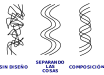
\includegraphics[width=0.55\textwidth]{img/composicion_1.png}
      \caption{Visualización de la separación de diferentes cosas y su composición}
      \label{fig_composicion_1}
   \end{center}
\end{figure}

\section{Extraer los cálculos de las acciones}
\noindent Observe la función \textit{grabar\_caudal()} que se muestra en el siguiente fragmento de código:

\vspace{0.7em}
\begin{Codigo}
   fn grabar_caudal() {
      let velocidad = leer_sensor();
      let caudal = 1.8 * velocidad.powf(3.2);
      save_caudal_to_database(caudal);
   }
\end{Codigo}

La función lee el valor de la velocidad de un sensor, realiza el cálculo del caudal asociado a esa velocidad y graba el resultado en una base de datos. La función es una acción: no tiene ningún argumento de entrada ni devuelve ningún resultado, pero tiene una entrada de datos implícita a través de la función \textit{leer\_sensor()} y una salida de datos implícita que graba datos en la base de datos utilizando la función \textit{save\_caudal\_to\_database()}.  

Además, la función incluye un cálculo, que aquí se ha expresado mediante una operación relativamente sencilla, pero que podría ser más complicado. 

Si se quisiera hacer algún test para comprobar que el cálculo se realiza de manera correcta, no sería fácil. Una opción sería habilitar el sensor correspondiente y la base de datos asociada mientras se hacen los test. Para comprobar que el resultado calculado es correcto, seguramente habría que consultar el valor grabado en la base de datos, pues la función no devuelve ningún valor. Si se quisiera probar el cálculo con diferentes valores de velocidad, habría que \textit{trucar} el sensor, lo que puede resultar complicado.

El problema está en que se están mezclando dos cosas: una acción (en ralidad, dos) y un cálculo. La solución adecuada es extraer el cálculo a una función independiente, como se muestra en el siguiente código:

\vspace{0.7em}
\begin{Codigo}
   fn grabar_caudal() {
      let velocidad = leer_sensor();
      
      let caudal = calcula_caudal(velocidad);
      
      save_caudal_to_database(caudal);
   }
   fn calcula_caudal(velocidad: f64) -> f64 {
      let resultado = 1.8 * velocidad.powf(3.2);
      resultado
   }
\end{Codigo}

Ahora hay dos funciones: una acción y un cálculo. Es fácil realizar los test para comprobar que los cálculos se hacen de manera adecuada. Se puede probar la función \textit{calcula\_caudal()} para cualquier valor de entrada de manera sencilla.

Los pasos que se han seguido se podrían esquematizar de la siguiente forma:
\begin{itemize}
   \item En la función original, seleccionar el fragmento de código a extraer.
   \item Ponerlo en una nueva función, sustituyéndolo en la función original por una llamada a la función recién creada. Es posible que haya que añadir algún parámetro.
   \item Identificar todas las entradas y salidas en la nueva función, convirtiendo las entradas en parámetros y las salidas en valores devueltos, que habrá que asignar a alguna variable en la función original.
   \item Los argumentos y lo valores devueltos de la función recién creadas tienen que ser inmutables, de forma que la nueva función sea un cálculo.
\end{itemize}

\section{Ejemplo: eliminar entradas implícitas}
\noindent En numerosas ocasiones, una misma función hace más de una cosa. Suponga que se tiene la siguiente función:

\vspace{0.7em}
\begin{Codigo}
   fn main() {
      facturar(100.0);
   }
   fn facturar(precio: f64) {
      let descuento = 0.10 * precio;
      println!("Precio      : {:.2}", precio);
      println!("Descuento   : {:.2}", descuento);
      println!("Precio neto : {:.2}", precio - descuento);
   }
\end{Codigo}

La función \textit{facturar()} recibe como argumento el precio de un artículo, calcula el descuento a aplicar y muestra el resumen de la factura en pantalla. Está haciendo dos cosas: calcular el descuento y mostrar los resultados en pantalla. El hecho de mostrar los resultados en pantalla es un efecto secundario, una salida implícita que convierte a la función en una acción. Pero, además, tiene una entrada implícita de información. El valor $0.10$ del porcentaje de descuento que se aplica es una especie de variable global, correspondiente a la lógica de negocio de la aplicación.

No es posible eliminar la acción, de hecho, es el objetivo del programa: mostrar la factura en pantalla, una vez que se ha aplicado el descuento. Es difícil diseñar un test para probar la función. Por una parte hay que probar que los cálculos son correctos y, por otra, que la salida de la función también es correcta. Tenga en cuenta que, aunque la salida se ha planteado simplemente mostrando unos mensajes en pantalla, podría tratarse de la actualización de ciertos registros en una base de datos o cualquier otra salida. En el caso de hacer la salida a una base de datos, para probar los cálculos, habría que habilitar y tener disponible la base de datos.

Lo correcto es separar el cálculo del descuento de la salida de resultados. Pero, además, la entrada implícita del porcentaje de descuento hay que convertirla en un parámetro de la función que calcula el descuento. Podría hacerse de la siguiente forma:

\vspace{0.7em}
\begin{Codigo}
   fn main() {
      let porcentaje_descuento = 0.10;
      let precio = 100.0;
      let descuento = 
      calcula_descuento(precio, porcentaje_descuento);
      facturar(precio, descuento);
   }
   fn calcula_descuento(precio: f64, porcentaje: f64) -> f64 {
      precio*porcentaje
   }
   fn facturar(precio: f64, descuento: f64) {
      println!("Precio      : {:.2}", precio);
      println!("Descuento   : {:.2}", descuento);
      println!("Precio neto : {:.2}", precio - descuento);
   }
\end{Codigo}

Ahora, la función \textit{calcula\_descuento()} es una función pura, un cálculo. Sus únicas entradas se producen a través de los argumentos que recibe y su salida es el valor que devuelve. No importa cuándo se llame a la función o cuántas veces se la llame: si recibe los mismos argumentos siempre devolverá el mismo resultado. Es fácil plantear los test para probar que realiza los cálculos de manera adecuada. 

Además, el porcentaje del descuento que se tiene que aplicar se ha independizado de cualquiera de las funciones. Está centralizado en una variable accesible para otras funciones del programa. Si la empresa decidiera cambiar su política de descuentos, solo tendría que modificar el valor de la variable en un sitio y se actualizaría la política en cualquier función que haga uso de ella.

Por otra parte, la función \textit{facturar()} sigue siendo una acción, pero independiente de otras consideraciones. Si se decidiera cambiar la forma de salida de la pantalla a una base de datos, por ejemplo, solo habría que actuar en dicha función, despreocupándose del cálculo de los valores asociados. Aun siendo una acción, se han eliminado sus entradas implícitas, convirtiéndolas en parámetros.

En el ejemplo, se han realizado varias refactorizaciones:
\begin{itemize}
   \item Extraer un cálculo de una acción.
   \item Convertir una entrada implícita en un parámetro.
   \item Separar las cosas en funciones independientes.
\end{itemize}

\section{Inmutabilidad. Copy-on-write}
\noindent Al inicializar una variable, se cambia su valor. Si en las funciones solo se inicializan variables locales, nada fuera de la función ve dichos cambios, salvo que lo vean a través del valor devuelto. 

Ejemplo sin copy-on-write:

\vspace{0.7em}
\begin{Codigo}
   fn main() {
      let mut list = vec![1, 2, 3];
      list.push(4);
      assert_eq!(list, vec![1, 2, 3, 4]);
   }
\end{Codigo}

Sin copy-on-write, pero con función:

\vspace{0.7em}
\begin{Codigo}
   fn main() {
      let mut list = vec![1, 2, 3];
      modify_list(&mut list, 4);
      assert_eq!(list, vec![1, 2, 3, 4]);
   }
   fn modify_list(list: &mut Vec<i32>, x: i32) {
      list.push(x);
   }
\end{Codigo}

Con copy-on-write:

\vspace{0.7em}
\begin{Codigo}
   fn main() {
      let list = vec![1, 2, 3];
      let list = copy_on_write(list, 4);
      assert_eq!(list, vec![1, 2, 3, 4]);
   }
   fn copy_on_write(list: Vec<i32>, x: i32) -> Vec<i32> {
      let mut new_list = list;
      new_list.push(x);
      new_list
   }
\end{Codigo}

No se modifica la lista original, se transforma en una nueva lista que incorpora las modificaciones. No hay pérdida de rendimiento, la propiedad de los valores se va trasmitiendo, sin modificar su posición en memoria.

Variante usando un \textit{RefCell}:

\vspace{0.7em}
\begin{Codigo}
   fn main() {
      let list = RefCell::new(vec![1, 2, 3]);
      let list = modify_cell(list, 4);
      assert_eq!(list.take(), vec![1, 2, 3, 4]);
   }
   fn modify_cell(list: RefCell<Vec<i32>>, x: i32) 
   -> RefCell<Vec<i32>> {
      let new_list = list;
      new_list.borrow_mut().push(x);
      new_list
   }
\end{Codigo}

\vspace{0.7em}
\begin{figure}[htb]
   \begin{center}
      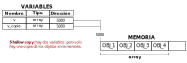
\includegraphics[width=0.8\textwidth]{img/shallow_copy.png}
      \caption{Esquema del mecanismo \textit{shallow-copy} de un \textit{array} en Java: se copian las referencias a los objetos, no los objetos en sí mismos. Al final hay dos variables apuntando a los mismos objetos en memoria.}
      \label{fig_shallow_copy_1}
   \end{center}
\end{figure}


\chapter{Colecciones}




\chapter{Patrones de diseño en la Programación Funcional}






\chapter{Grokking Simplicity}

\IndiceCapitulo

\begin{Resumen}   
   {\color{blue}Apuntes del Libro <<Grokking Simplicity>>, de Eric Norman \citep{normandGrokkingSimplicityTaming2021}}
\end{Resumen}

\section{Welcome to Grokking simplicity}

\section{Functional thinking in action}

\section{Distinguishing actions, calculations and data}

Los programadores funcionales clasifican cualquier fragmento de código como acción, cálculo o datos. Esta clasificación puede recibir otras denominaciones, pero el concepto es el mismo. 

\begin{itemize}
   \item \textbf{Acciones:} son todo aquello que dependa de en qué momento se ejecuta o de cuántas veces se ejecuta. Por ejemplo, enviar un correo es una acción.
   \item \textbf{Cálculos:} son las tareas que solo dependen de los valores de entrada para generar un resultado. Los cálculos siempre devuelven el mismo resultado, si los valores de entrada son los mismos. Además, los cálculos nunca afectan a nada que esté fuera de ellos. Esto hace que los cálculos sean fáciles de testear y que su uso sea seguro, pues no hay que preocuparse de cuántas veces se utilicen o en qué orden sean invocados: si los parámetros de entrada son los mismos, el resultado será siempre el mismo.
   \item \textbf{Datos:} los datos son información registrada acerca de los acontecimientos. Tienen propiedades conocidas. Un mismo dato se puede interpretar de manera diferente según el contexto de ejecución en el que se encuadra. Por ejemplo, la factura de una cena la puede utilizar el cliente para llevar la cuenta de sus gastos mensuales o la puede utilizar el propietario del restaurante para determinar los gustos favoritos de sus clientes.
\end{itemize}

\begin{figure}[htb]
   \centering
   \includegraphics[width=0.7\linewidth]{img/AccCalcData.png}
   \caption{Ejemplos de código: Acciones, Cálculos y Datos}
   \label{fig_acccalcdata}
\end{figure}


La proliferación de los sistemas distribuidos en los que intervienen diferentes dispositivos y peticiones cuasi simultáneas de información a las bases de datos, el problema de organizar de manera adecuada el código se hace indispensable. En general, el código de las acciones será más difícil de comprender y de testear que el código de los cálculos, ya que estos últimos no dependen del número de veces que se invocan o del orden de dichas invocaciones. Es por ello que se hace importante separar en la medida de los posible el código que corresponde a las acciones del código que corresponde a los cálculos.

La programación funcional proporciona herramientas para el correcto tratamiento de cada una de estas categorías de código. En el caso de las acciones, es importante gestionar la forma en que cambia el estado de las variables del programa a lo largo del tiempo, garantizando el número de veces y el orden en el que se realiza cada acción. Los cálculos tienen su propia estrategia para comprobar su buen funcionamiento, a veces basada en técnicas matemáticas. En el caso de los datos, es importante organizarlos en estructuras que faciliten un acceso eficiente a la información que se quiere extraer de los mismos.

Hay dos técnicas fundamentales que permiten abordar los programas con un enfoque funcional: 
\begin{itemize}
   \item Distinguir en el código las acciones, de los cálculos y los datos.
   \item Utilizar abstracciones de primera clase.
\end{itemize}

A lo largo del curso se tratará de trasmitir el razonamiento funcional a la hora de abordar un problema de codificación. El objetivo es que las técnicas que se aprendan sean independientes del lenguaje que se utilice para programar y que sean de aplicación inmediata, tanto para la realización de un programa nuevo, como para refactorizar partes de un código ya existente.

Para clasificar el código en acciones, cálculos y datos es útil seguir los principios del \textit{diseño estratificado}, separando el código en diferentes capas. Para organizar el orden en el que se ejecutan las acciones son de utilidad los \textit{diagramas de tiempos} y la utilización de funciones de \textit{primera clase}, que permiten utilizar otras funciones como parámetros o resultados.

En el diseño estratificado, se organiza el código en diferentes capas, ordenadas en función de la mayor o menor probabilidad de cambios en el código correspondiente a lo largo de la vida útil de la aplicación. Se suelen considerar tres capas principales:

\begin{itemize}
   \item \textbf{Nivel técnico:} correspondería a la parte de la aplicación que tiene menos probabilidades de cambiar. Por ejemplo, el lenguaje de programación de la aplicación o las estructuras de datos que se utilizarán para almacenar la información.
   \item \textbf{Reglas del dominio de la aplicación:} si por ejemplo se está haciendo una aplicación para gestionar unos cultivos de hortalizas, las distancia optima a la que hay que poner las plantas en el terreno o la cantidad de humedad que necesitan corresponden al campo de conocimiento de dicho dominio técnico y es difícil que cambien durante la vida útil de la aplicación.
   \item \textbf{Reglas del negocio:} se consideran aquí reglas que vienen marcadas por la aplicación concreta que se esté desarrollando. En el ejemplo de los cultivos podrían ser los precios de los factores de producción o la disponibilidad de determinados recursos.
\end{itemize}

Cada capa de la aplicación se desarrolla sobre las demás y solo debe depender de las capas que hay situadas por debajo de ella. De esta forma, si se produce una modificación en algún elemento, se sabe que solo puede afectar a los elementos que estén situados en la misma capa o en las capas superiores. La Figura \ref{fig_stratified} muestra un ejemplo de organización en capas de una aplicación para gestionar cultivos.

\vspace{1em}
\begin{figure}[htb]
   \centering \fbox{
      \includegraphics[width=0.8\textwidth]{img/stratified.png}
   }
   \caption{Esquema de capas en el diseño estratificado}
   \label{fig_stratified}
\end{figure}

\subsection{Líneas de tiempos}
En todas las aplicaciones hay que establecer el orden en el que se tienen que realizar las acciones. En aplicaciones sencillas, una distribución secuencial de las acciones puede ser suficiente. Pero, en sistemas distribuidos, en los que distintas tareas pueden correr a cargo de distintos componentes que pueden trabajar en paralelo o de forma concurrente, es importante establecer el orden en el que se tienen que realizar todas las acciones y los puntos en los que determinadas acciones no pueden ejecutarse si antes no se ha finalizado determinada acción anterior. Hay que cortar la línea de tiempos en algunos puntos para indicar que la ejecución no puede continuar hasta que se completen todas las tareas anteriores.

La Figura \ref{fig_timeline_1} muestra la línea de tiempos de una aplicación en la que, para poder ejecutarse las acciones \textit{D} y \textit{E} es necesario que primero se hayan completado las tareas llevadas a cabo por los componentes \textit{A}, \textit{B} y \textit{C}.

\vspace{1em}
\begin{figure}[htb]
   \centering \fbox{
      \includegraphics[width=0.65\textwidth]{img/timeline_1.png}
   }
   \caption{Cortando la línea de tiempo para garantizar el orden de ejecución de las acciones}
   \label{fig_timeline_1}
\end{figure}

La línea de tiempos ayuda a coordinar distintas acciones y a determinar los puntos en los que se pueden producir cuellos de botella durante la ejecución de los programas en sistemas distribuidos.

\section{Distinción entre acciones, cálculos y datos}
Antes de ponerse a codificar una aplicación nueva, conviene razonar .para distinguir qué elementos del programa serán acciones, cálculos o datos. En general, el orden de implementación consistirá en definir primero los datos, luego los cálculos y, por último, las acciones.

Cuando se está analizando un código ya existente, habrá que identificar igualmente las funciones que incluyen acciones. En muchos casos, una misma función incluirá acciones y cálculos. En esos casos, conviene refactorizar para separar las acciones de los cálculos.  

Como se ha comentado, las acciones dependen de cuándo se ejecutan o de cuantas veces se ejecutan. Las funciones que implementan acciones se suelen denominar \textit{funciones impuras} o \textit{funciones con efectos secundarios}. Enviar un correo o leer datos de una base de datos serían ejemplos de acciones.

Por el contrario, los cálculos solo dependen del valor de los parámetros de entrada y no producen efectos secundarios. Se denominan \textit{funciones puras} o \textit{funciones matemáticas}. Calcular el máximo de una serie de números o comprobar si determinada dirección de correo es válida podrían ser ejemplos de funciones puras. 

Se dice que los cálculos son \textit{referencialmente trasparentes}. La trasparencia referencial significa que se puede sustituir el cálculo por el resultado sin que el programa se vea afectado. Por ejemplo, si una función realiza la suma de dos números, en los lugares del programa donde se hace la llamada a la función se puede sustituir ésta por el resultado de la suma y el programa no se verá afectado.

Los datos son hechos.

\subsection{Entradas y salidas implícitas}
\noindent Los parámetros de una función son el procedimiento de \textit{entrada explícita} de datos a la función. El valor devuelto por la función es la salida \textit{explícita}. 
Cuando una función es impura, tiene entradas o salidas implícitas. Se denomina \textit{entrada implícita} a la entrada de datos a la función que no procede de un parámetro. Se denomina \textit{salida implícita} al valor que sale de la función sin hacerlo a través del valor devuelto por la misma.

El código del ejemplo muestra una función denominada \textit{contador\_impuro()} que no tiene parámetros ni devuelve ningún valor. En cambio, la función recibe como entrada implícita el valor de un contador existente en la base de datos, a través de un método llamado \textit{get\_contador\_from\_database()}, y realiza una salida también implícita reescribiendo en la base de datos el valor incrementado de dicho contador a través del método \textit{update\_contador\_in\_database()}. La salida implícita de la función es, además, un efecto secundario de la misma, convirtiendo a dicha función en una \textit{acción}.

\begin{EjemploCodigo}[Entradas y salidas implícitas]{ejimplicita1}
   fn contador_impuro() {
      let contador = get_contador_from_database(); // Entrada implícita
      update_contador_in_database(contador+1); // Salida implícita
   }
\end{EjemploCodigo}

El acceso a variables globales dentro de una función es una forma de entrada o salida implícita.

En la medida de lo posible, hay que evitar las entradas y salidas implícitas, pues complican la trazabilidad y la facilidad de testeo de las funciones. En muchas ocasiones, las entradas implícitas se pueden sustituir por parámetros de la función. De la misma forma, las salidas implícitas es posible sustituirlas por valores devueltos por las funciones.


\section{Ejemplo}

\begin{EjemploCodigo}[Ejemplo carrito]{}
   struct Producto {
      name: String,
      precio: f64,
   }
   fn main() {
      let mut carrito = Vec::<Producto>::new();
      let mut total_compra: f64 = 0.0;
      let producto = Producto{name: "Sandalias".to_string(), precio: 12.5};
      add_producto(producto, &mut carrito, &mut total_compra);
   }
   fn add_producto(producto: Producto, carrito: &mut Vec<Producto>, total_compra: &mut f64) {
      carrito.push(producto);
      calc_total_carrito(carrito, total_compra);
   }
   fn calc_total_carrito(carrito: &mut Carrito, total_compra: &mut f64) {
      *total_compra = 0.0;
      for producto in &carrito.items {
         *total_compra = *total_compra + producto.precio;
      }
      actualiza_web_total_compra( *total_compra);	
   }
   fn actualiza_web_total_compra(total_compra: f64) {  }
\end{EjemploCodigo}

\section{Extracting calculations from actions}
\section{Improving the design of actions}
\section{Staying inmutable in a mutable language}
\section{Staying inmutable with untrusted code}


\section{Stratified design (I)}
\section{Stratified design (II)}
\section{First-class functions (I)}
\section{First-class functions (II)}
\section{Functional iteration}
\section{Chaining functional tools}
\section{Functional tools for nested data}
\section{Isolating timelines}
\section{Sharing resources between timelines}
\section{Coordinating timelines}
\section{Reactive and onion architectures}
\section{The functional journey ahead}


%\begin{EjemploCodigo}[]{}
%\end{EjemploCodigo}

%
%
%\begin{EjemploCodigo}[]{}
%	
%\end{EjemploCodigo}

\chapter{Functional Programming made easier (Scalfani)}

\section{1.- Discipline is freedom}
\subsection{Global State}
\noindent El uso de varibles globales conlleva determinados inconvenientes:
\begin{itemize}
   \item Cualquiera desde cualquier módulo puede cambiar el valor de las variables globales.
   \item Se producen acoplamientos de las variables globales entre sí y de unos módulos con otros.
   \item En programación concurrente no hay garantías respecto de la modificación de las variables.
   \item Colisión de nombres entre las variables globales y otros identificadores en cualquier módulo.
\end{itemize}

En el caso de la programación orientada a objetos se produce la misma circunstancia con el patrón \textit{Singleton}.

Los lenguajes de PF prohíben la existencia de variables globales. Rust permite solo la existencia de constantes globales.

\subsection{Mutable State}
\noindent La posibilidad de que las variables puedan cambiar de valor también tiene algunos inconvenientes. Por ejemplo, es más difícil razonar sobre el código, pues los valores que pueden cambiar pueden hacer cambiar también la semántica del programa, o hacer el código más frágil.

En los lenguajes funcionales, las variables son inmutables y ello da lugar a algunas consecuencias.
\begin{itemize}
   \item Las expresiones del tipo $x = x +1$ no tienen sentido. Una vez que se asigna un valor a $x$, no se puede cambiar.
   \item Las asignaciones como $x=20$ son \textit{expresiones referencialmente trasparentes}, esto es, en cualquier parte del programa se puede utilizar indistintamente $x$ o $20$ con la seguridad de que el programa seguirá funcionando igual. La trasparencia referencial permite una evaluación \textit{lazy} de la sustitución de $x$ por su valor en el código.
\end{itemize}

Si las variables no pueden cambiar de estado, no es posible hacer bucles. En los lenguajes funcionales, los bucles se sustituyen por la recursividad. Cualquier bucle se puede ejecutar mediante recursividad y viceversa.

Por ejemplo, la definición matemática del factorial de un número se podría hacer de la siguiente forma:
\begin{equation}
   \label{eq_factorial_1}
   n! = 1.2...(n-2).(n-1).n \quad \forall n \in \mathds{N} 	
\end{equation}
Con esta definición, parecería inmediato resolver el problema con un bucle, como se hace en el Ejemplo \ref{ejfactorial1}.

\vspace{1em}
\begin{EjemploCodigo}[Factorial calculado con un bucle]{ejfactorial1}
   fn factorial_bucle(n: u32) -> u32 {
      let mut prod = 1;
      for i in 1..=n {
         prod = prod*i;
      }
      prod
   }
\end{EjemploCodigo}

Si en la Expresión \ref{eq_factorial_1} se cambia el orden del producto, los términos se podrían agrupar de la siguiente manera:
\begin{equation}
   \label{eq_factorial_2}
   n! = n.(n-1)...2.1 \quad = n . (n-1)! \quad \forall n \in \mathds{N} 	
\end{equation}

Con esta definición surge el problema de calcular $0!$, pero su valor se puede deducir. De la Expresión \ref{eq_factorial_1} se sabe que $!1 = 1$. Se podría operar de la siguiente forma:
\begin{align*}
   1! &= 1 \\
   1! &= 1. (1-1)! = 1 . 0! \\
   1  &= 1 . 0! = 0! \\
\end{align*}

Con lo que finalmente queda que:
\begin{equation}
   \label{eq_factorial_3}
   0! = 1
\end{equation}
Una vez calculado el valor de $0!$, se puede proceder a definir el factorial de cualquier número natural con la siguiente definición recursiva:
\begin{align} \label{eq_factorial_4}		
   0! &= 1 \nonumber \\
   n! &= n . (n-1)! \quad \forall n \in \mathds{N} 
\end{align}

Esta definición de factorial se podría codificar como se hace en el Ejemplo \ref{ejfactorial2}.

\vspace{1em}
\begin{EjemploCodigo}[Factorial calculado de manera recursiva]{ejfactorial2}
   fn factorial_recursivo(n: u32) -> u32 {
      match n {
         0 => 1,
         _ => n*factorial_recursivo(n-1)
      }
   }
\end{EjemploCodigo}



\section{Variables globales}
\noindent Vamos a ver en primer lugar cómo no se pueden usar las variables globales en Rust. Podríamos estar tentados de usar sentencias \textit{let}, como en la variables locales de cualquier función:

\vspace{0.7em}
\begin{Codigo}
   use chrono::Utc;
   
   let START_TIME: String = Utc::now().to_string();
   
   fn main() {
      ...
   }
\end{Codigo}

El código anterior no compila, no se pueden usar asignaciones \textit{let} en el ámbito global, pues la instrucción \textit{let} crea una variable en la memoria stack, que no se inicializa hasta que se ejecuta el programa. Las variables globales solo se pueden crear utilizando las cláusulas \textit{const} o \textit{static}, que utilizan la memoria del segmento de datos (\textit{data segment}) del programa. 

Tampoco se puede compilar la siguiente inicialización:

\vspace{0.7em}
\begin{Codigo}
   use chrono::Utc;
   
   static START_TIME: String = Utc::now().to_string();
   
   fn main() {
      ...
   }
\end{Codigo}

El compilador avisa que no se pueden utilizar funciones no constantes en la inicialización de variables globales. No se puede ejecutar ningún tipo de código antes de que el programa comience. El valor de una variable global debe ser conocido en el momento de la compilación, antes de la ejecución. 

Tampoco valdría declarar la variable global y tratar de asignarle valor en \textit{main()}:

\vspace{0.7em}
\begin{Codigo}
   use chrono::Utc;
   
   static START_TIME: String;
   
   pub fn main() {
      START_TIME =  = Utc::now().to_string();
      println!("{}", START_TIME);
   }
\end{Codigo}

El código anterior tampoco compila, el compilador nos avisa de que hay que asignar algún valor a la variable \textit{static}. Podríamos pensar en asignarle un valor \textit{None}

\vspace{0.7em}
\begin{Codigo}
   use chrono::Utc;
   
   static mut START_TIME: Option<String> = None;
   
   pub fn main() {
      START_TIME = Some(Utc::now().to_string());
      println!("{}", START_TIME);
   }	
\end{Codigo}

Pero el código anterior tampoco compila, el compilador nos avisa de que una variable global mutable solo se puede utilizar dentro de un bloque inseguro \textit{unsafe{}}. Finalmente, si encerramos el código dentro de \textit{main()} en un bloque \textit{unsafe{}}, sí que compila:

\begin{Codigo}
   use chrono::Utc;
   
   static mut START_TIME: Option<String> = None;
   
   pub fn main() {
      unsafe{
         START_TIME =  Some(Utc::now().to_string());
         println!("{}",  START_TIME.clone().unwrap());
      };
   }
\end{Codigo}

Ahora, el código compila y se puede ejecutar, pero no parece una forma muy cómoda de utilizar, aunque en algunas ocasiones pudiera ser útil.

Vamos a ver otro problema relacionado con la extensión del dominio de las variables. En un programa como el anterior, no se necesitaría declarar la variable como global, se podría declarar dentro de la función \textit{main()}. Pero suponga que lo que se quiere es utilizar la variable en un hilo diferente creado dentro de \textit{main()}

\begin{Codigo}
   use chrono::Utc;
   
   pub fn main() {
      let start_time = Utc::now().to_string();
      
      let thread_1 = std::thread::spawn(||{
         println!("Started {}, called thread 1 {}", &start_time, Utc::now());
      });
      
      thread_1.join().unwrap();
   }
\end{Codigo}

Si tratamos de compilar este código, el compilador nos dirá que el hilo \textit{thread\_1} podría vivir más tiempo que la variable \textit{start\_time} que se ha creado en el marco de datos en el stack de la función \textit{main()} y no está garantizado que la variable sobreviva lo suficiente. Nosotros, viendo el código, sabemos que al hacer el \textit{join()} antes de salir de \textit{main()} estamos garantizando esa supervivencia, pero el compilador no nos deja compartir con otros hilos variables que no tengan una vida útil \textit{\&static}.

Hay un par de soluciones posibles sin utilizar variables globales. La primera sería clonar la variable \textit{start\_time} y pasar a la closure la propiedad del valor clonado:

\begin{Codigo}
   pub fn main() {
      let start_time = Utc::now().to_string();
      let cloned_start_time = start_time.clone();
      let thread_1 = std::thread::spawn( move ||{
         println!("Started {}, called thread 1 {}", &cloned_start_time, Utc::now());
      });
      thread_1.join().unwrap();
   }	
\end{Codigo}

Esta solución puede servir para una variable de cadena de caracteres como la anterior, pero si hubiera que clonar una variable de mayor tamaño podría no ser la solución óptima. En esos casos se podría envolver la variable con un puntero \textit{Arc}:



\begin{Codigo}
   use chrono::Utc;
   use std::sync::Arc;
   
   pub fn main() {
      let start_time = Arc::new(Utc::now().to_string());
      let cloned_start_time = Arc::clone(&start_time);
      let thread_1 = std::thread::spawn(move ||{
         println!("Started {}, called thread 1 {}", &cloned_start_time, Utc::now());
      });
      
      thread_1.join().unwrap();
   }
\end{Codigo}

Si además se necesitara mutabilidad interior de la variable, se podría envolver en un \verb+ Arc<Mutex<String>>+.

\subsection{Valor conocido en tiempo de compilación}
\noindent Cuando el valor de la variable global se conoce en tiempo de compilación, hay básicamente dos soluciones:
\begin{itemize}
   \item \textbf{const:} valores constantes que se conocen en tiempo de compilación. No permiten la mutabilidad interior. El compilador resuelve sustituyendo el valor en línea (inline)\footnote{Conviene consultar el apartado de la cláusula \textit{const} en la documentación en  \url{https://doc.rust-lang.org/std/keyword.const.html} y del concepto de \textit{expresiones constantes} en \url{https://doc.rust-lang.org/reference/const_eval.html}}. 
   \item \textbf{static:} las variables reciben un espacio de memoria en el segmento de datos. Es posible la mutabilidad interior.
\end{itemize}

Si se necesita mutabilidad interior, para los tipos primitivos se pueden utilizar valores \textit{atomic} \footnote{Ver libro en líne de Mara Bos \url{https://marabos.nl/atomics/}} y, para tipos más complejos, se pueden usar \textit{locks} en la forma \textit{read-write lock}, \textit{RwLock} o en la forma \textit{mutual exclusion lock}, \textit{Mutex}. 

Si lo que se necesita es calcular el valor en tiempo de ejecución, las soluciones con \textit{const} y \textit{static} no sirven.

\chapter{Railway Oriented Programming}

El \textit{Railway Oriented Programming} es un término acuñado por Scott Wlaschin que propone un modelo del tratamiento de errores en la programación funcional.

\begin{itemize}
   \item Railway Oriented Programming: \url{https://fsharpforfunandprofit.com/rop/}
   \item Monoids without tears: \url{https://fsharpforfunandprofit.com/posts/monoids-without-tears/}
\end{itemize}

\section{Monoides}

\textbf{Morfismo:} en varios campos de las matemáticas, se llaman \textit{morfismos} (u \textit{homomorfismos}) a las aplicaciones entre estructuras matemáticas que preservan la estructura interna. Por ejemplo, en teoría de conjuntos, los morfismos son las aplicaciones entre conjuntos; en álgebra lineal, las transformaciones lineales; y en topología, las funciones continuas. En \textit{teoría de las categorías}, el morfismo tiene una noción más general.

\textbf{Categoría:} una categoría viene dada por dos tipos de datos: una clase de objetos y, para cada par de objetos X e Y, un conjunto de morfismos desde X hasta Y. En el caso de una categoría concreta, X e Y son conjuntos de cierto tipo y un morfismo \textit{f} es una función desde X a Y que satisface alguna condición.

Los morfismos se representan frecuentemente como flechas entre los objetos. Esto origina la notación:
\begin{equation}
   f : X \rightarrow Y   
\end{equation}



\chapter{NaN an Inf}

\url{https://stackoverflow.com/questions/14682005/why-does-division-by-zero-in-ieee754-standard-results-in-infinite-value}

\section{Artículos para recomendar a los alumnos}
The Mediocre Programmer's Guide to Rust:

{\footnotesize \url{https://www.hezmatt.org/~mpalmer/blog/2024/05/01/the-mediocre-programmers-guide-to-rust.html} \par}

